%
% Projekt: proj4.tex
% Autor:   Michal Ľaš
% Datum:   11.04.2023
% 


\documentclass[a4paper, 11pt, a4paper]{article}
\usepackage[left=2cm,text={17cm, 24cm},top=3cm]{geometry}

\usepackage[slovak, english]{babel}
\usepackage{times}
\usepackage[utf8]{inputenc}
\usepackage[T1]{fontenc}
\usepackage[hidelinks]{hyperref}
\usepackage{url}
\usepackage{graphicx}

\graphicspath{{../images/}}
%\DeclareUrlCommand\url{\def\UrlLeft{<}\def\UrlRight{>} \urlstyle{tt}}


\begin{document}


\begin{titlepage}
    \begin{center}
            \textsc{\Huge Brno University of Technology \\}
            \vspace{0.5em}
            \textsc{\huge Faculty of Information Technology \\}
        \vspace{\stretch{0.382}}
            {\LARGE Microprocessors and Embedded Systems\,--\,Project \\ 
            \vspace{0.4em}
            \Huge Bluetooth Metronome}
        \vspace{\stretch{0.618}}
    \end{center}
    {\Large \today \hfill Michal Ľaš (xlasmi00)}
\end{titlepage}

% Table of contents
\tableofcontents
\newpage

% Body
\section{Introduction}

The project's objective was to develop a metronome tailored for musicians, with Bluetooth functionality for remote control.
The chosen platform for implementation was the ESP32 chip. The metronome was designed to offer adjustable settings for speed, 
volume, and rhythm. Users can easily control these parameters through a simple HTML interface, leveraging the capabilities 
of Web Bluetooth technology.

The resulting application was created using the C programming language and the \texttt{esp-idf} framework. Primary references for this project 
were derived from the \texttt{esp-idf} documentation \cite{esp.guide} and examples available in the esp-idf GitHub repository \cite{esp.idf}, as well as various online sources. 
Notably, resources from the websites about web bluetooth technology \cite{JS.BLE} and insights on Web Bluetooth, Generic ATTribute (GATT), and  
Generic Access Profile (GAP) \cite{BLE.guid} played a key role in shaping the implementation.

\section{Hardware connection}

GPIO pin 14 serves as the control interface for the external buzzer, as illustrated in Figure \ref{figure:buzzer.connection}. Simultaneously, 
the built-in LED, located on GPIO pin 2, is utilized in the system. In the event of a successful client connection to the device, 
the integrated LED flashes three times as an indicator.

\begin{figure}[ht]
    \begin{center}
        \scalebox{0.6}{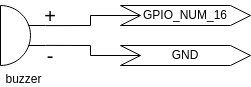
\includegraphics{../images/hw-connection.png}}
    \end{center}
    \caption{Buzzer connection to ESP32}
    \label{figure:buzzer.connection}
\end{figure}


\section{Design}

The project can be divided into 2 parts:\\

\noindent\textbf{1. Metronome Control:}

\begin{itemize}
    \item The metronome's tempo, regulated by a GPTimer (General Purpose Timer), ensures periodic ticking. This timer triggers a buzzer sound event, managed through the \verb|init_metronome_timer()| function.
    \item The metronome can be activated with \verb|run_metronome()| and halted with \verb|stop_metronome()|. To set the tempo (BPM), use \verb|set_metronome_tempo(bpm)|.
    \item Before commencing the metronome, it is essential to initialize Pulse Width Modulation (PWM) for GPIO pin 14 (buzzer pin) using the \verb|pwm_init()| function.
    \item Buzzer triggering and volume are modulated using \verb|set_duty_cycle(duty)|, while the buzzer's frequency or tone is adjusted with \verb|set_buzzer_frequency(frequency)|.
\end{itemize}

\noindent\textbf{2. Bluetooth Communication:}

\begin{itemize}
    \item The \verb|init_ble()| function kickstarts Bluetooth Low Energy (BLE) settings and initiates a thread for capturing Bluetooth events. Two UUIDs, one for Bluetooth service and another for Bluetooth characteristic, were generated using the UUID generator tool \cite{UUID.gen}. 
    \item \verb|ble_app_advertise()| initiates device advertising. Upon client connection, \verb|ble_gap_event()| captures and signals a successful connection by flashing the built-in LED thrice this function also handles device disconnection. Upon disconnection, the application reinitiates advertising, enabling the establishment of another connection. This ensures continuous accessibility for potential users seeking to connect with the device.
    \item Messages from the client are intercepted by \verb|ble_gatt_event()|, with processing managed by the \verb|write_client()| function. This establishes comprehensive control over all metronome functions for the client.
\end{itemize}

\noindent This configuration empowers the client to have comprehensive control over all the metronome functions outlined earlier.

Additionally, the implementation features a client comprising a straightforward HTML page (refer to image \ref{figure:api}) accompanied 
by a script, \texttt{script.js}. This script is responsible for messaging to manipulate the metronome. Each message starts with the 
first byte denoting the action code, succeeded by supplementary data. For example, to establish the tempo, the code is \texttt{0x30}, 
followed by the tempo value. This messaging protocol ensures a structured and efficient means for the client to convey instructions 
to control various metronome parameters.\\

\noindent\textbf{Codes:}

\begin{itemize}
    \item \texttt{0x30}: Set tempo message
    \item \texttt{0x31}: Set rhythm/beat message
    \item \texttt{0x32}: Set volume message
    \item \texttt{0x33}: Start metronome message
    \item \texttt{0x34}: Stop metronome message
    \item \texttt{0x35}: Initialize metronome values (set metronome at connection)
\end{itemize}

\begin{figure}[ht]
    \begin{center}
        \scalebox{0.4}{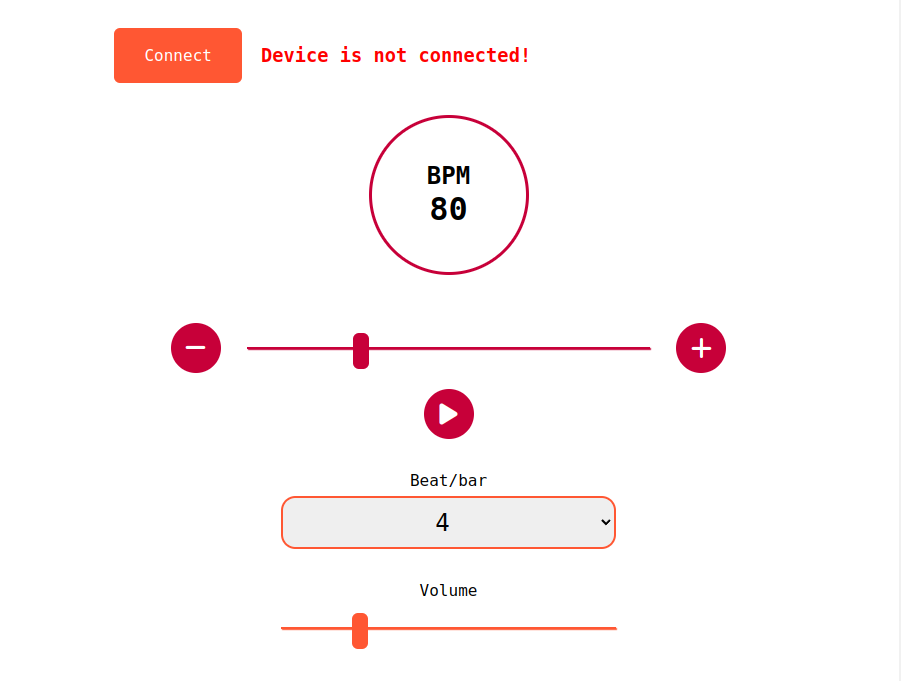
\includegraphics{../images/api.png}}
    \end{center}
    \caption{Bluetooth Metronome Client API}
    \label{figure:api}
\end{figure}

\section{Requirements}

\begin{itemize}
    \item ESP32 with bluetooth
    \item ESP-IDF Release v5.1.2 or newer
    \item Chrome browser (version 119.0 or newer)
\end{itemize}


\section{Limitations and known bugs}

\begin{itemize}
    \item BLE functionality is operational within secure contexts, necessitating the use of the HTTPS protocol for the client application. Simple HTTP without TLS is not supported. (application can be deployed also on localhost)
    \item BLE is working only in secure contexts. So it needs to use HTTPS protcol for a client application (it works on localhost as well). Simple HTTP without TLS is not supported.
    \item The \verb|+| and \verb|-| buttons in the client application currently lack an implemented debounce timer. Consequently, rapid button presses may result in collisions, wherein a previously sent message is not processed before the next one arrives (this issue manifests only when the client is actively connected to the device). 
\end{itemize}


\section{Conclusion}

The project managed to implement all the assignment points.



% Literature
\newpage

\bibliographystyle{enplain.bst}
\renewcommand{\refname}{Literature}
\bibliography{documentation}

\end{document}
